%-------------------------------------------------------------------------------
% THIS FILE IS AN EXAMPLE ON HOW TO USE THE "revstat-v2.sty" PACKAGE...
% last modified: 2019/12/02
%-------------------------------------------------------------------------------
% REVSTAT - STATISTICAL JOURNAL
% Instituto Nacional de Estat�stica - Portugal
% https://www.ine.pt/revstat/inicio.html
% revstat@ine.pt
%-------------------------------------------------------------------------------
% The following 10 packages are pre-loaded:
%
%     graphicx   latexsym   enumerate   amsmath   amsfonts   amssymb
%     amsthm     amsopn     amstext     amscd     lineno     hyperref
%-------------------------------------------------------------------------------
\documentclass[twoside,leqno,11pt]{article}
\usepackage{revstat-v2}
%\usepackage{lastpage}
\begin{document}
%%%%%%%%%%%%%%%%%%%%%%%%%% alteracao %%%%%%%%%%%%%%%%%%%%%%%%%%%%%%%%%%
\thispagestyle{firstpage}

\vspace{-3.2cm}

\noindent
{\footnotesize {\sffamily REVSTAT~~--~~Statistical~~Journal\\[-1pt]
Volume 0, Number 0, Month 0000,
 000-000}}
% \thepage-\pageref{LastPage}}}   % requires \usepackage{lastpage}

\vspace{1.5cm}
%%%%%%%%%%%%%%%%%%%%%%%%%% alteracao %%%%%%%%%%%%%%%%%%%%%%%%%%%%%%%%%%
%-------------------------------------------------------------------------------
% Title of the article...
%-------------------------------------------------------------------------------
\title{TITLE - NO MORE THAN 120 CHARACTERS (WITH SPACES) - THIS FILE IS AN EXAMPLE ON HOW TO USE THE ``REVSTAT-V2.STY'' PACKAGE
%\footnote{The opinions expressed in this text are those of the authors and do not necessarily reflect the views of any organization.}
}
\renewcommand{\titleheading}
             {Using the ``revstat-v2.sty" Package}  % --- on odd running heads
%-------------------------------------------------------------------------------
% Author(s)' names and addresses...
%-------------------------------------------------------------------------------
\author{\authoraddress{Author Abcdefg
\href{https://orcid.org/0000-0004-8882-8330}{
\includegraphics[scale=0.08]{ORCID-iD_icon-128x128}}
                        \correspondingauthor} % Corresponding author
                       {Some Department,
                       Some University,\\
                       A Planet Earth Country
                       \ (author.abcdefg@org.country)}
\\
        \authoraddress{Author Hijklmn \href{https://orcid.org/0000-0004-8882-8330}{
\includegraphics[scale=0.08]{ORCID-iD_icon-128x128}}}
                      {Some Organization Department,
                       Some Institute,\\
                       Another Planet Earth Country
                       \ (author.hijklmn@org.country)}
}
\renewcommand{\authorheading}
             {Author Abcdefg \ and \ Author Hijklmn}  % --- on even running heads

%-------------------------------------------------------------------------------
% Just asking LaTeX to effectively do the title...
%-------------------------------------------------------------------------------
\maketitle
%-------------------------------------------------------------------------------
% Just asking LaTeX to numerate lines...
%-------------------------------------------------------------------------------
\setpagewiselinenumbers
\modulolinenumbers[1]
\linenumbers
%%%%%%%%%%%%%%%%%%%%%%%%%% alteracao: Datas %%%%%%%%%%%%%%%%%%%%%%%%%%%%%%%%%%
\noindent
~~~~{\small{\sffamily Received:} Month 0000 ~~~~~~{\sffamily Revised:} Month 0000 ~~~~~~{\sffamily Accepted:} Month 0000}
%%%%%%%%%%%%%%%%%%%%%%%%%% alteracao %%%%%%%%%%%%%%%%%%%%%%%%%%%%%%%%%%

%-------------------------------------------------------------------------------
% Abstract of the article...
%-------------------------------------------------------------------------------
\begin{abstract}
A summary of less than one hundred words, followed by a maximum of six key words and the AMS 2000 subject classification. The paper should not have more than 25 pages. If necessary authors may consider a file for Supplementary Material, from their own responsibility. This paper approaches issues related with frame problems and nonresponse in surveys. These
\emph{nonsampling errors}  % --- to emphasize text use \emph{}
affect the accuracy of the estimates whereas the estimators become biased and less precise. We analyse some estimation methods that deal with those problems and give an especial focus to the poststratification procedures. We then address the Bootstrap methodology for variance estimation.
\end{abstract}

%-------------------------------------------------------------------------------
% Keywords...
%-------------------------------------------------------------------------------
\begin{keywords}
Poststratification; frame problems; nonresponse; reweighting; adjustment methods; Bootstrap.
\end{keywords}

%-------------------------------------------------------------------------------
% AMS classifications...
%-------------------------------------------------------------------------------
\begin{ams}
49A05, 78B26.
\end{ams}


%-------------------------------------------------------------------------------
% Main text of the paper:  sections, subsections and subsubsections,
%                          with theorems, lemmas, ..., figures, tables, ..., etc
%-------------------------------------------------------------------------------
%%%%%%%%%%%%%%%%%%%%%%%%%% alteracao %%%%%%%%%%%%%%%%%%%%%%%%%%%%%%%%%%
%\mainpaper  % --- just a blank page and a \newpage command
\newpage     % --- just a newpage - not a blank page
%%%%%%%%%%%%%%%%%%%%%%%%%% alteracao %%%%%%%%%%%%%%%%%%%%%%%%%%%%%%%%%%
%-------------------------------------------------------------------------------
% First section
%-------------------------------------------------------------------------------
\section{INTRODUCTION}  % --- sections in UPPERCASE
\label{Sec1}              % --- this section label

The importance of the treatment of factual items in the XYZ has long been recognized in the literature\footnote{See, for instance, Rothwell (\cite{R1}).}.
If not excluded for the purposes of index number compilation, the most common approaches to the treatment of such goods are the so-called fix...


\section{DESCRIPTION OF THE PROBLEM}
\label{Sec2}

\subsection{Theoretical background}

As mentioned in section~\ref{Sec1}, in principle, the difficulties raised by the existence of factual items can be tackle by either:
\begin{enumerate}
\item[a)] ignoring the issue and excluding all the possible `problematic' items from XYZ compilation;
\item[b)] allocating fixed weights, assuming that factual items are to be treated in the same way as all other items (this is the fixed weights approach);
\item[c)] allocating variable/changing weights, according to the consumption pattern found in the base year (this is the variable weights approach).
\end{enumerate}

Table~\ref{Tab1} summarises the main advantages and disadvantages of the three considered approaches.

\vspace*{5mm}
\begin{table}[h]
\centering
\begin{tabular}{|c|c|c|}
\hline
\textbf{Approach} & \textbf{Advantages} & \textbf{Disadvantages}\\
\hline
Ignore... & Simplicity & Overlooking...\\
Fixed-weight & Theoretical consistency & Choice of imputation... \\
Variable-weight & Minimisation... & Theoretical inconsistency\\
\hline
\end{tabular}
\caption{Advantages and disadvantages of different approaches to the treatment of factual items in a XYZ.
\label{Tab1}}
\end{table}
\vspace*{5mm}

Ignoring the `problematic' or more `volatile' items can be seen as a non-solution in the context of an index that wants to reflect changes in consumption prices. If these items have some importance in the XYZ basket, then there is, in principle, no reason for ignoring them.

Figure~\ref{Fig1} compares the carry forward and percentage change indices.\break
Although different in level, they nearly have the same turning points and behaviour in terms of movement.

\vspace*{5mm}
\begin{figure}[h]
\centering
%\includegraphics{rs-fig01.eps}
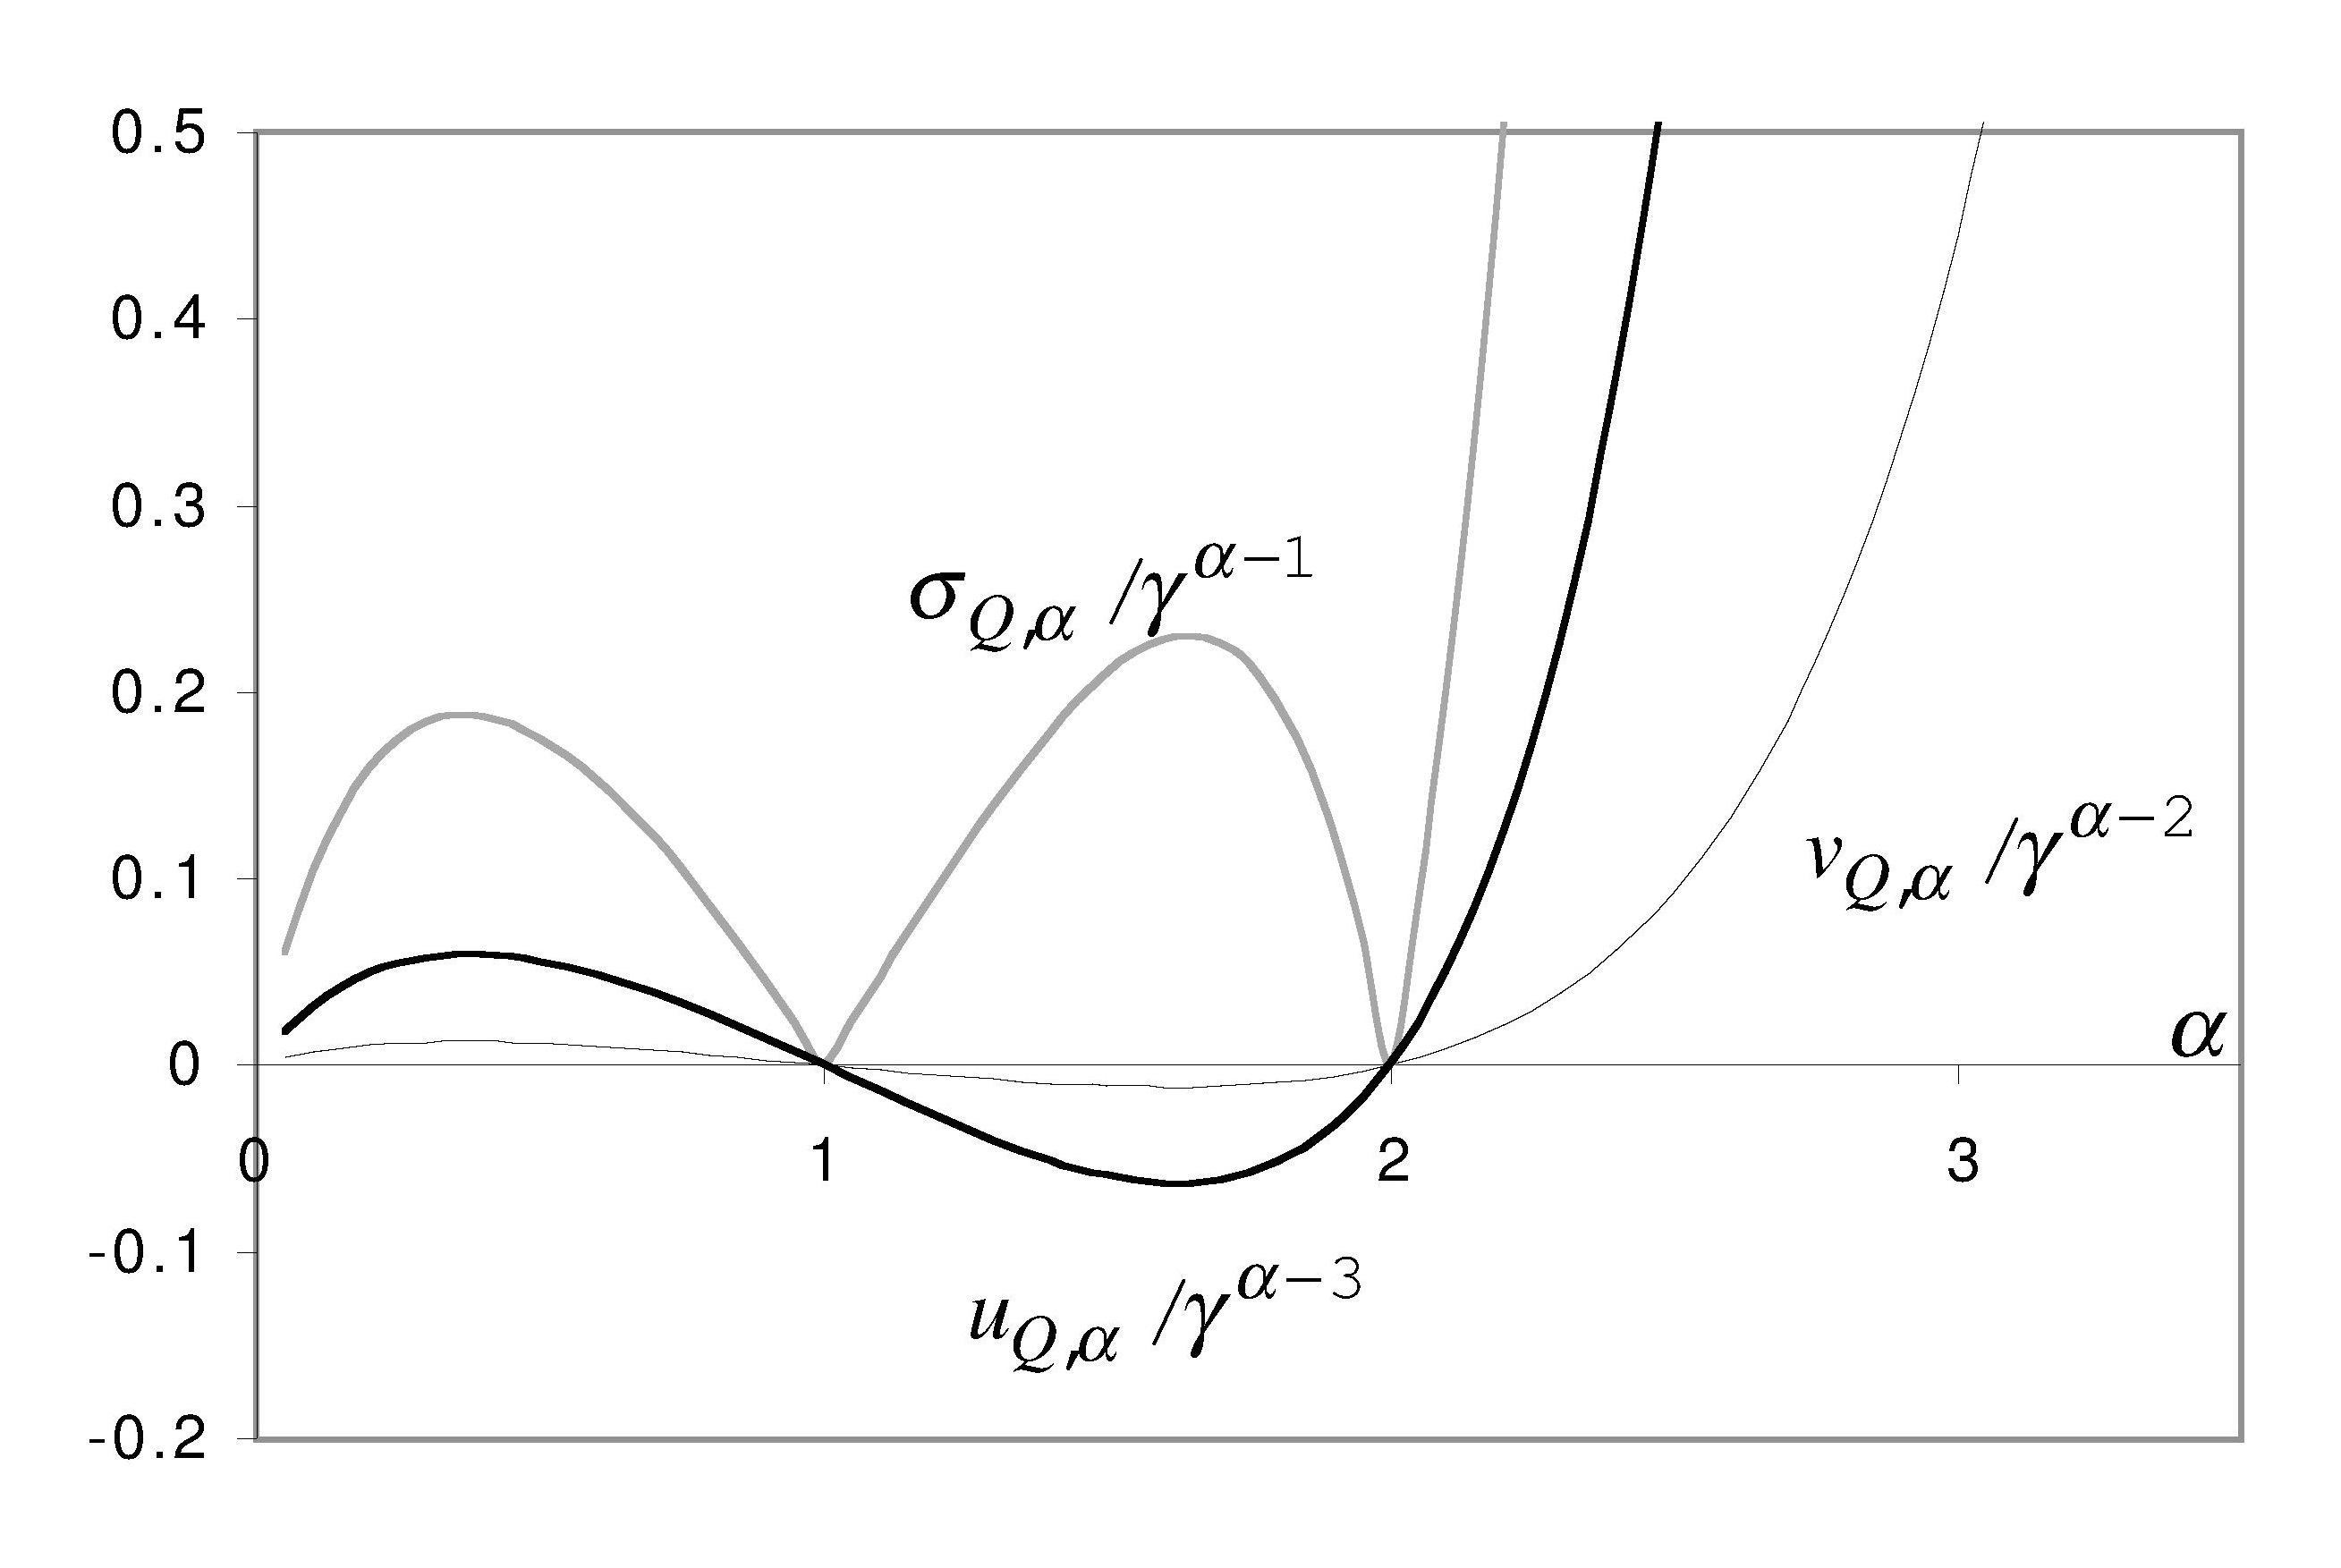
\includegraphics[width=0.7\textwidth]{rs-fig01.png}
\caption{Carry forward and percentage change indices.\hfil\break
Both indices tend to approximate in the months with less prices.
 \label{Fig1}}
\end{figure}
\vspace*{5mm}

\begin{theorem}
\label{Thm1}
Consider aggregation with all the other XYZ components.
\begin{equation}
\label{Eq1}
I_{i;o,m}^{t,m}=\frac{p_{i;t,m}}{p_{i;o,m}}~.
\end{equation}
\end{theorem}

\begin{proof}
This could be the proof of the previous Theorem...
\end{proof}


\subsubsection{This is a subsubsection}

The percentage change index presents a higher volatility than the forward imputation method (\ref{Eq1}), (\ref{Eq2}) and (\ref{Eq3}) (see Theorem~\ref{Thm1} and Lemma~\ref{Lem1}).

\begin{lemma}
\label{Lem1}
Consider aggregation with all the other XYZ components. That is only possible at the class level:
\begin{eqnarray}
\label{Eq2}
 && I_{i;o,m}^{t,m}=\frac{p_{i;t,m}}{p_{i;o,m}}~,~~~~m,n\in\N~;\\[2mm]
\label{Eq3}
 && {}_{s}I_{o,m}^{t,m}=\sum_{i}I_{i;o,m}^{t,m}\,
 \frac{p_{i;t,m}\cdot q_{i;o,m}}{{\displaystyle \sum_{i} p_{i;t,m}\cdot q_{i;o,m}}}~.
\end{eqnarray}
\end{lemma}

No matter which approach is followed, one has to bear in mind that no ``perfect" solution exist...
\\\\
Similar environment for corollary, proposition, ...
%\begin{corollary} \label{Cor1}
% First Corollary...
% \end{corollary}

%\begin{proposition} \label{Pro1}
% First Proposition...
% \end{proposition}

\begin{remark}
\label{Rem1}
First Remark...
\end{remark}

% \begin{note} \label{Not1}
% First Note...
% \end{note}
\noindent
Similar  environment for note, definition, example, ...

% \begin{definition} \label{Def1}
% First Definition...
% \end{definition}

% \begin{example} \label{Exa1}
% First Example...
% \end{example}

\begin{proof}[Proof of Lemma~\ref{Lem1}]
This is the proof of the previous Lemma...
\end{proof}

%-------------------------------------------------------------------------------
% Acknowledgments... Changed in revstat-v2
%-------------------------------------------------------------------------------
\begin{acknowledgments}
This work has been supported by the grant number xyz from Research Institution XX.
We also acknowledge the valuable suggestions from Prof.\ EFG and the referees.
\end{acknowledgments}
%-------------------------------------------------------------------------------
% References...
%-------------------------------------------------------------------------------
\begin{thebibliography}{8}

% --- example of Journal article:
\bibitem{Ab1}
\textsc{Author, B.}
 (1980).
 Article title in lowercase,
\textit{Journal Name In Uppercase},
\textbf{23},
 4,
 230--350.

\bibitem{R1}
\textsc{Rothwell, D.P.}
 (1958).
 Use of varying seasonal weights in price index construction,
\textit{Journal of the American Statistical Association},
\textbf{53}, 1, 66--77.

% --- example of Book:
\bibitem{Ab2}
\textsc{Author, B.} (1990).
\textit{Book Name In Uppercase}, Academic Press, New York.

\bibitem{Ro1}
\textsc{Robert, C.P.} (1999).
\textit{Monte Carlo Statistical Methods}, Springer Verlag.

% --- example of contribution on Book:
\bibitem{Ab3}
\textsc{Author, B.}  (2000).
\textit{Contribution title in lowercase}.
 In "Book Name In Uppercase"
 (J.\ Black and A.\ White, Eds.),
 Academic Press, New York, 123--130.

\bibitem{Ru1}
\textsc{Runbin, D.G.}
 (1988).
\textit{Using the SIR algorithm to simulate posterior distributions}.
 In ``Bayesian Statistics"
 (J.M.\ Bernardo, ... and A.F.M.\ Smith, Eds.),
 Oxford University Press, 395--402.

% --- example of 2 authors (book):
\bibitem{AA1}
\textsc{Author, B.\ \textup{and} Author, C.}  % --- notice the upshape "and"
 (1980).
\textit{Book Name In Uppercase},
 Academic Press, New York.

% --- example of 3 or more authors (book):
\bibitem{AAA1}
\textsc{Author, B.; Author, C.\ \textup{and} Author, D.}  % --- ";" and "and"
 (1980).
\textit{Book Name In Uppercase},
 Academic Press, New York.

\end{thebibliography}


\end{document}
